\documentclass{beamer}

\usepackage[utf8]{inputenc}
\usepackage{amsmath}
\usepackage{graphicx}
\usepackage{booktabs}
\usepackage{caption}
\usepackage{pgfplots}
\usepackage{multicol}
\usepackage{pgfplotstable}
\usepackage{pgf}
\usepackage{import}

\begin{document}
\begin{frame}
	\frametitle{ROM for BGK equation}
	\framesubtitle{BGK velocityspace}
	Original snapshot data in velocity space at time $t_{end}$.
	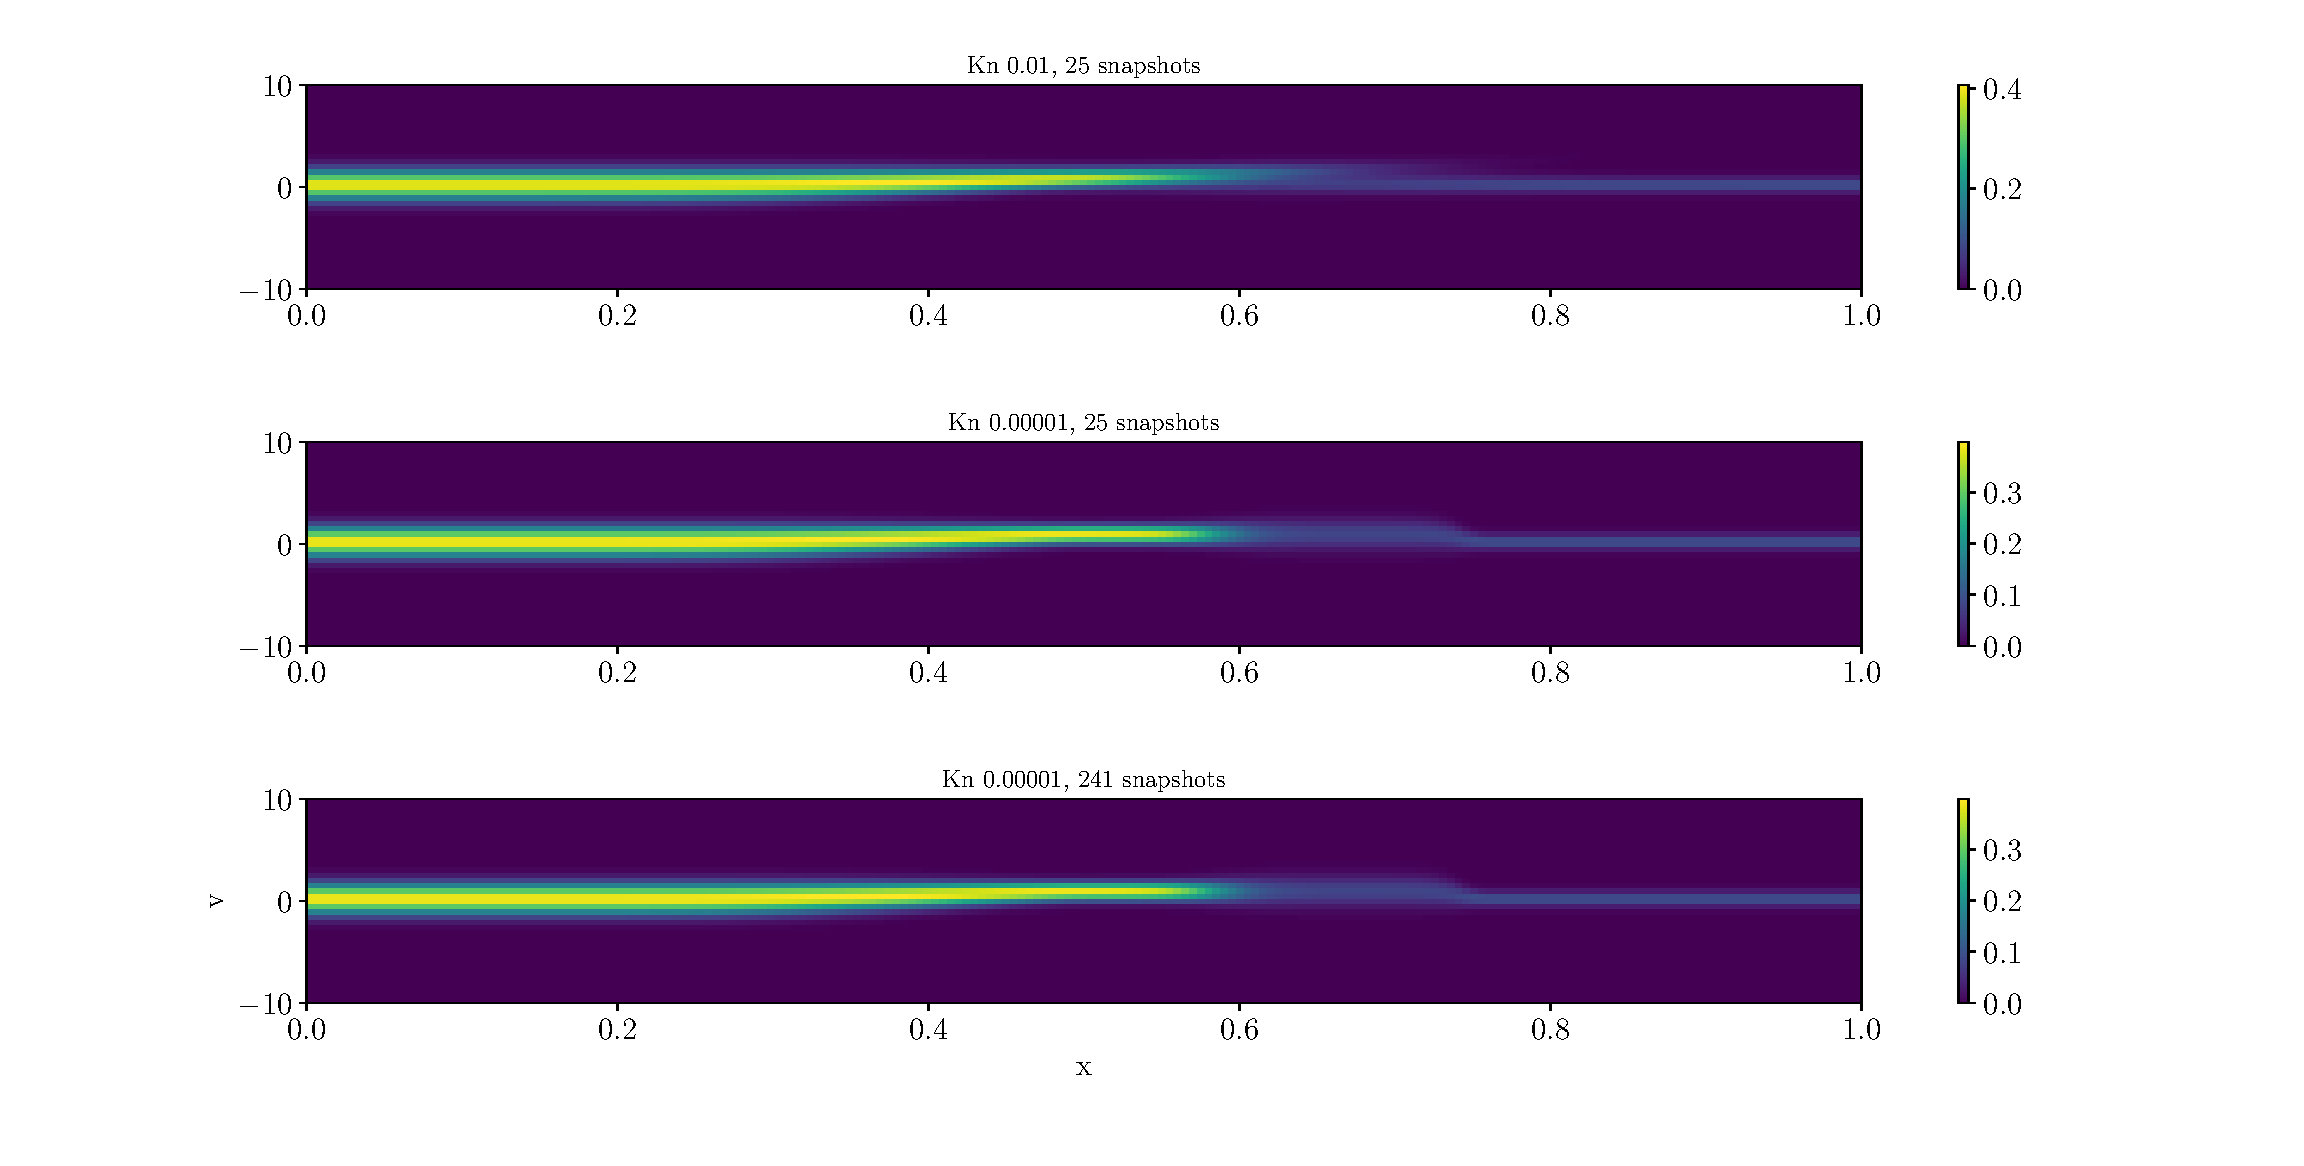
\includegraphics[width=1.1\textwidth]{figures/VelocitySpace.pdf}
\end{frame}
\begin{frame}
	\frametitle{ROM for BGK equation}
	\framesubtitle{Eckard-Young Theorem and snapshot matrix S}
	Alignment of tensorvalued data $f^{t \times v \times x}$ into an 2D-array S for decomposition:
		\[S = \begin{bmatrix}
		f_{1}(\xi_{1})&f_{2}(\xi_{1})&\cdots &f_{N_{snaps}}(\xi_{1}) \\
		f_{1}(\xi_{2})&f_{2}(\xi_{2})&\cdots &f_{N_{snaps}}(\xi_{2}) \\
		\vdots & \vdots & \ddots & \vdots\\
		f_{1}(\xi_{N_{\xi}})&f_{2}(\xi_{N_{xi}})&\cdots &f_{N_{snaps}}(\xi_{N_{\xi}})
		\end{bmatrix}\]
		\begin{itemize}
			\item The SVD decomposes the data into three unitary matrices $S=U\Sigma V^{*}$
			\item Eckart-Young Theorem : The optimal rank-r approximation to S, in a least squares sense, is given by the rank-r SVD truncation $\hat{S}$: argmin $||S-\hat{S}||_{F}=\hat{U}\hat{\Sigma}\hat{V}^{*}$
		\end{itemize}
\end{frame}
\begin{frame}
		\frametitle{ROM for BGK equation}
		\framesubtitle{Cumulative energy and singular values}
		Comparison of of the singular values $\sigma_{k}$ for the microscopic and macroscopic data with $\Sigma = diag(\sigma_{k})$.
		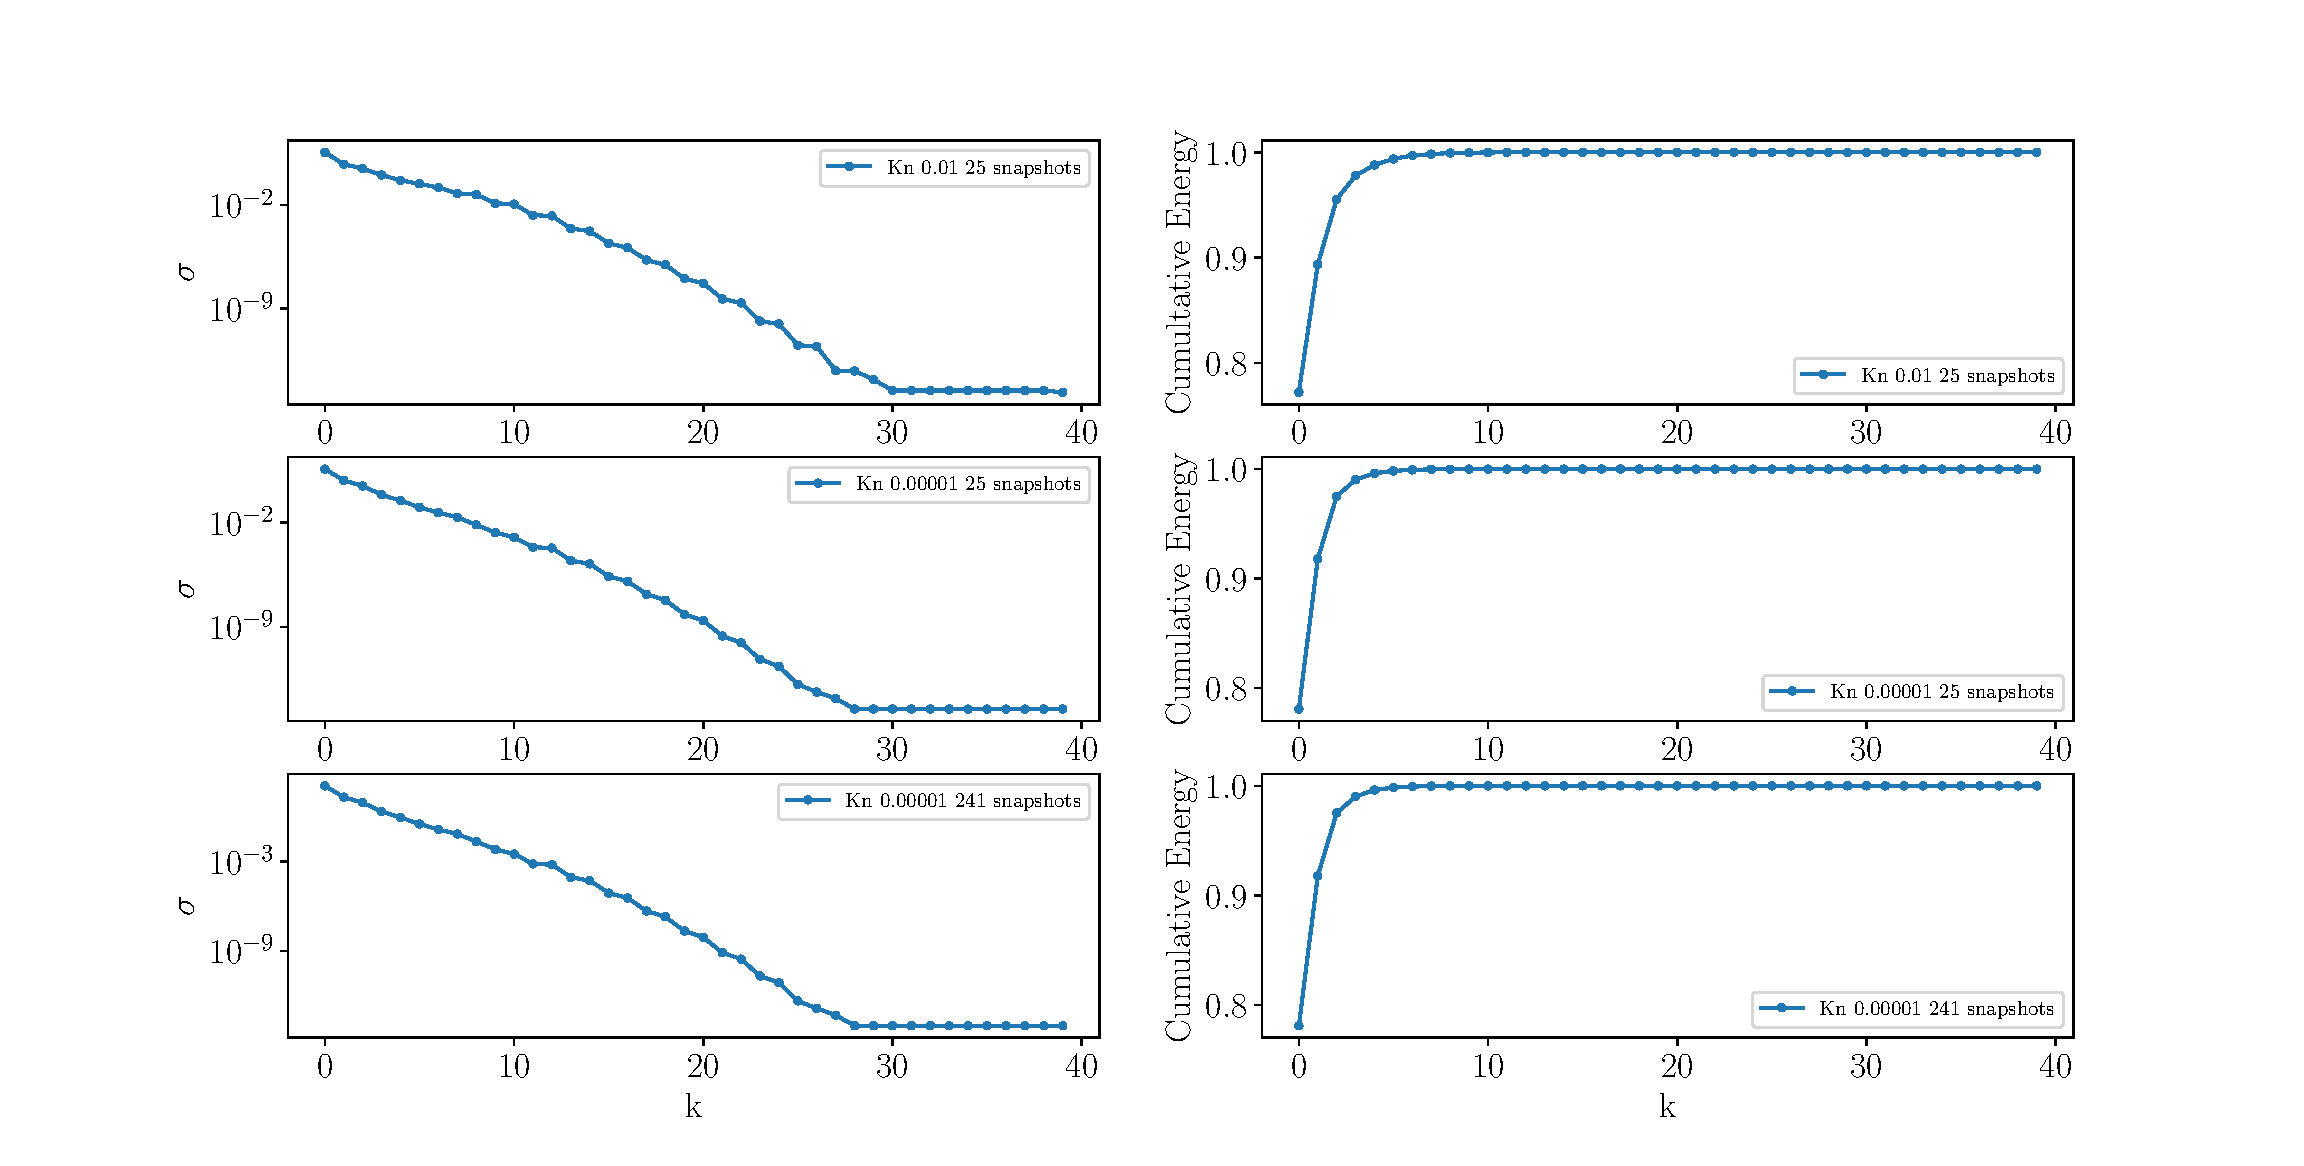
\includegraphics[width=1.\linewidth]{figures/Cumulative_sum.pdf}
		Cumulative sum of given data $\{a,b,c\}\rightarrow a, a+b, a+b+c$
\end{frame}
\begin{frame}
		\frametitle{ROM for BGK equation}
		\framesubtitle{Eigenmodes of the microscopic data} 
			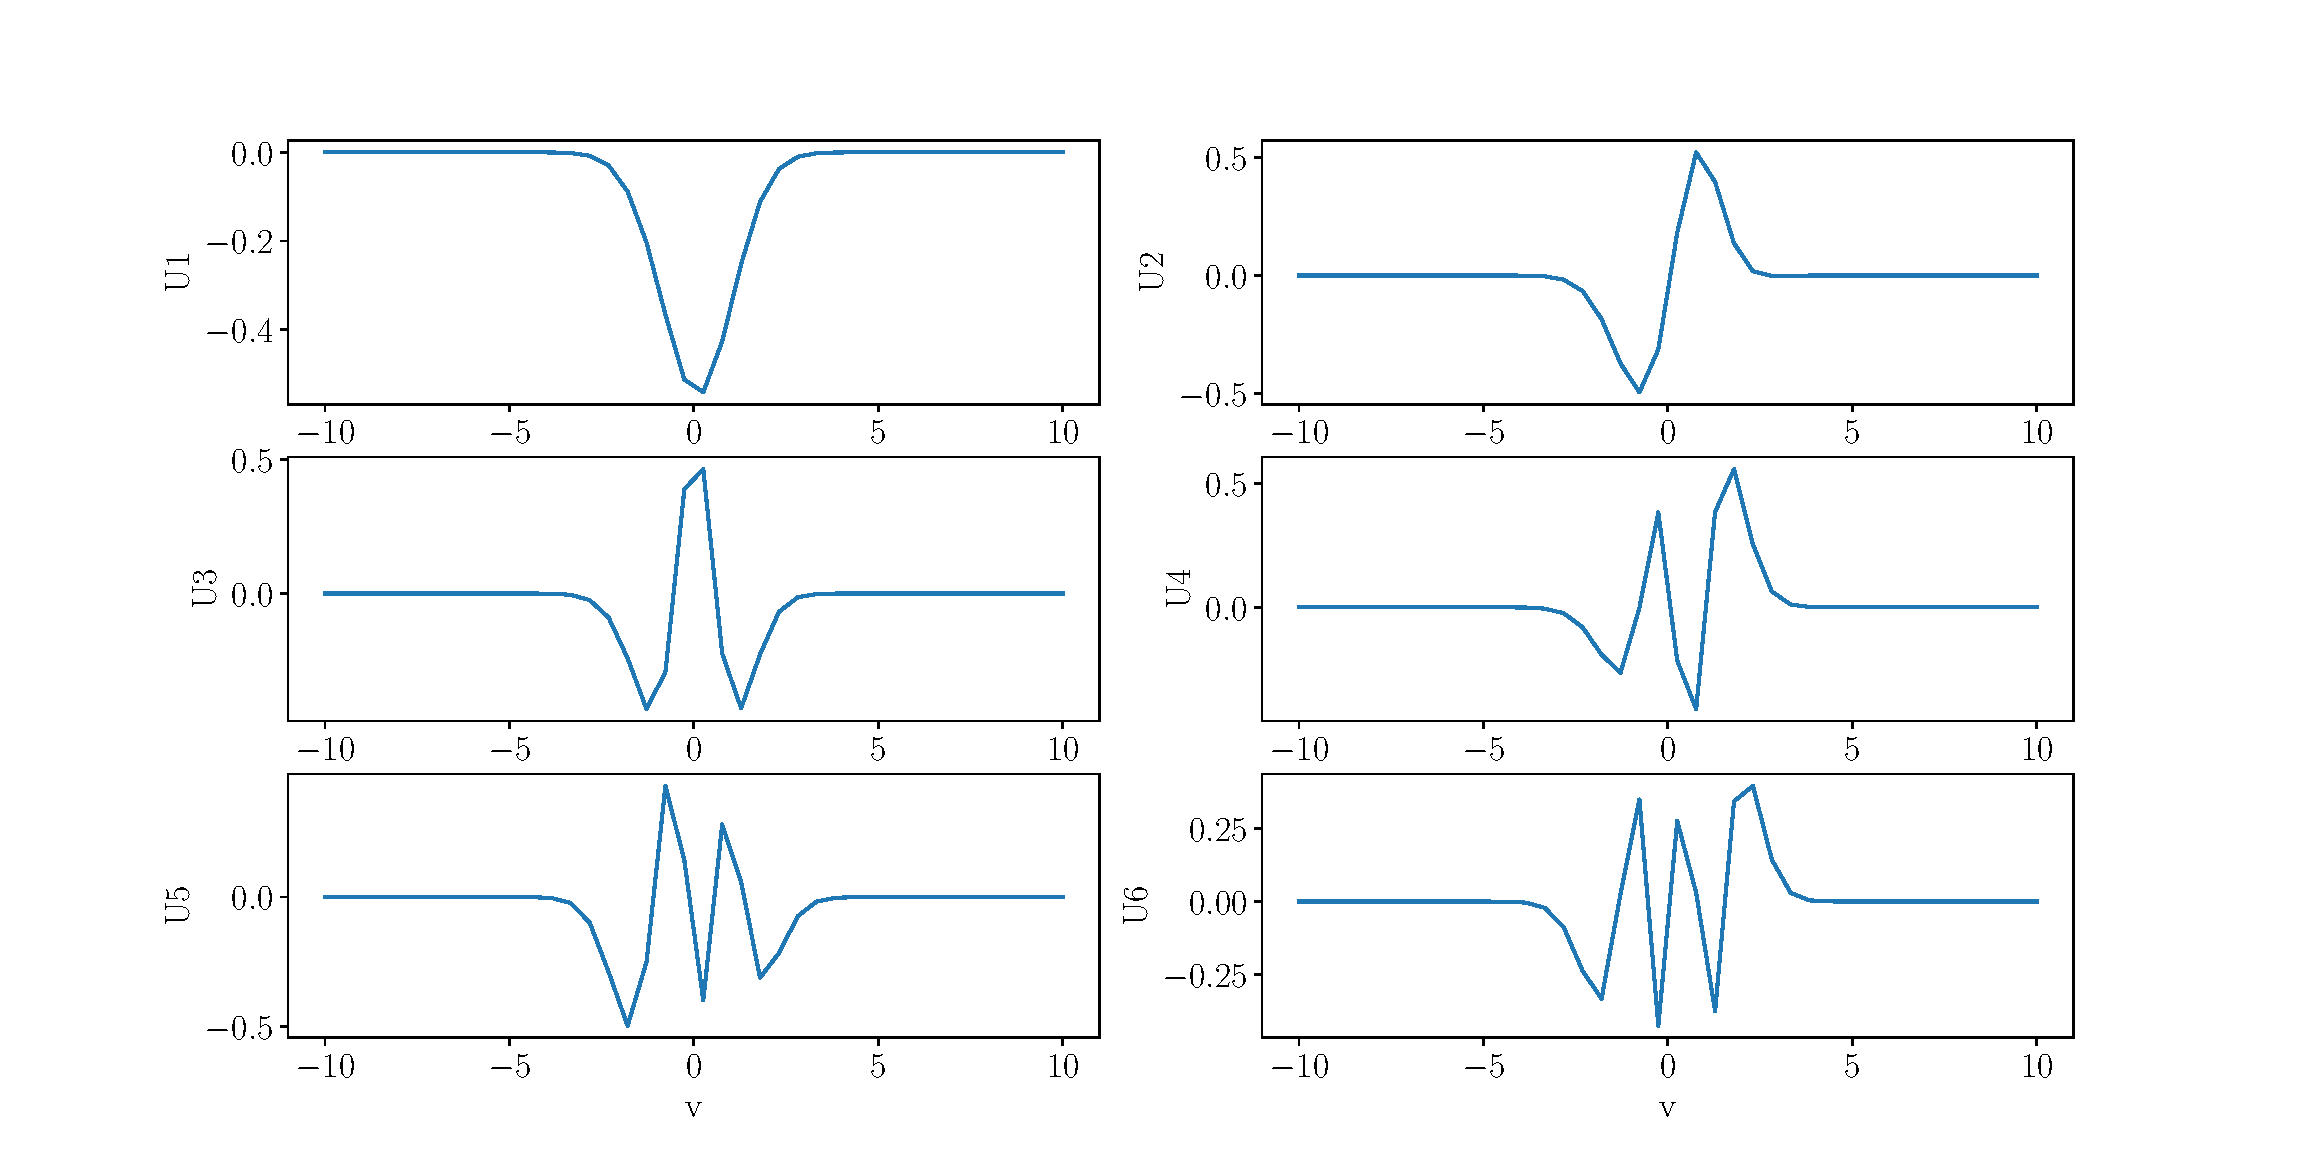
\includegraphics[width=\textwidth]{figures/SixModes25Kn0p01.pdf}
\end{frame}
\begin{frame}
		\frametitle{ROM for BGK equation}
		\framesubtitle{Eigenmodes of the macroscopic data.}
		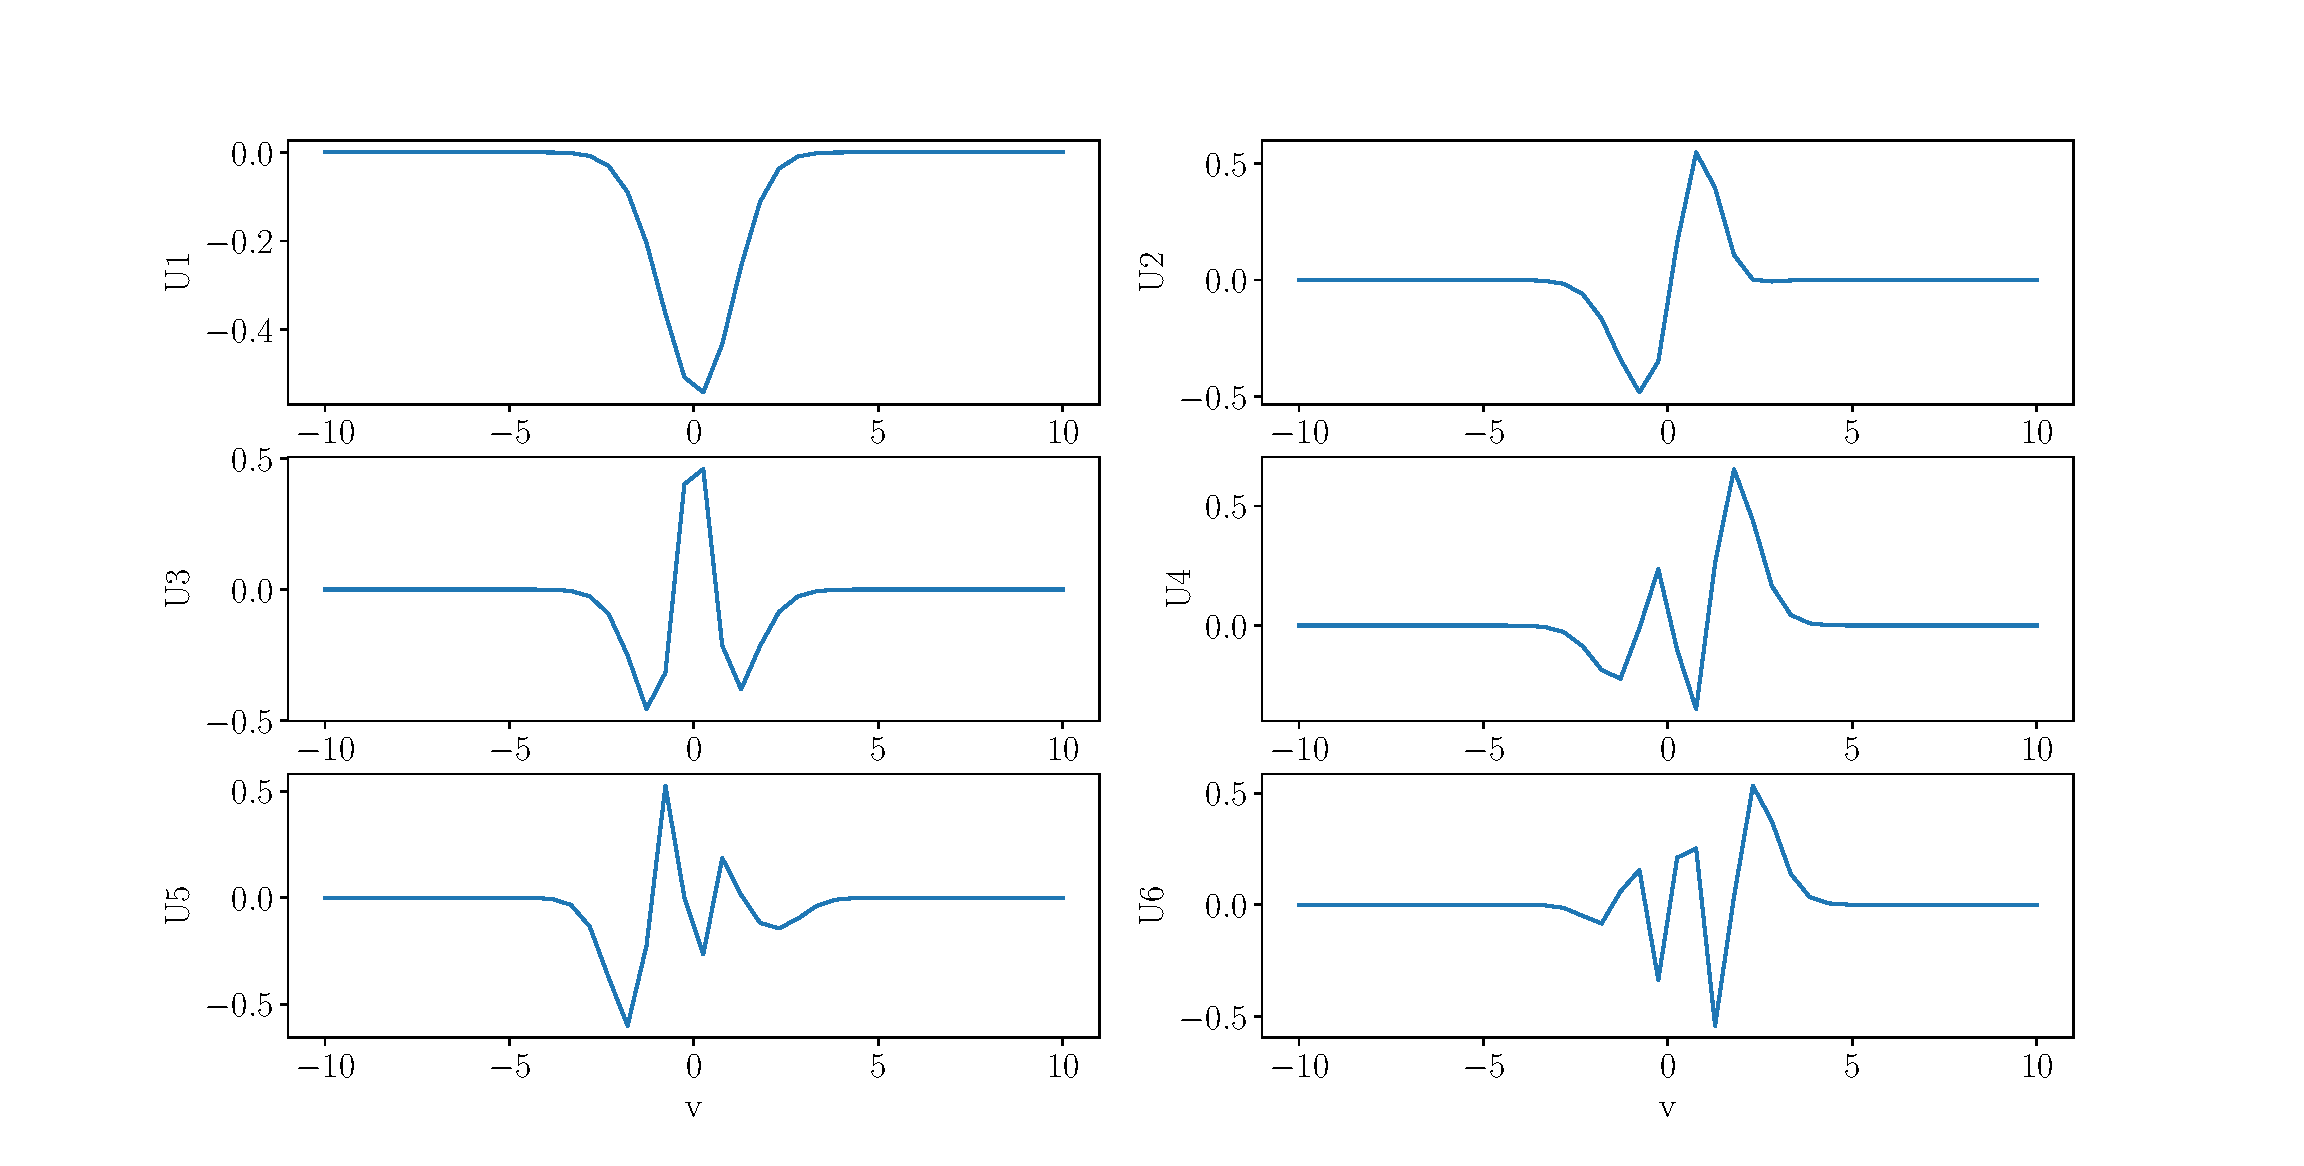
\includegraphics[width=\textwidth, height=\textheight,keepaspectratio]{figures/SixModes241Kn0p00001richtig.pdf}
\end{frame}
\begin{frame}
		\frametitle{ROM for BGK equation}
		\framesubtitle{Compressed Data}
		Density over x for the compressed (dotted red) and original (blue) data at time $t_{end}$. The compressed data consists of the first three eigenmodes.
	\includegraphics[width=\textwidth, height=0.6\textheight]{figures/TruncDens.pdf}
\end{frame}
\end{document}